\section{Séries temporais e a tarefa de predição}


\setcounter{subsection}{-1}
\subsection{Normalização dos dados}

	De acordo com enunciado disponibilizado, os dados devem ser normalizados de
	maneira a obter média nula e desvio padrão unitário. Entradas que excursionam
	em intervalos muito extensos prejudicam o desempenho das redes neurais MLP.
	
	\vspace{12pt}
	
	Sendo assim, faremos uso da seguinte equação para atingir as características
	necessárias:
	
	\begin{equation}
	X_i = \frac{V_i - \hat{\mu}}{\hat{\sigma}}
	\end{equation}
	
	em que \(\hat{\mu}\) é a média de todas as entradas (calcula através de
	\texttt{mean(dengue\_SP)}) e \(\hat{\sigma}\) é o estimador do desvio padrão
	(calculado por \texttt{std(dengue\_SP)}). Obtem-se, assim, um novo vetor cuja
	média e variância valem, respectivamente, \(1.8288\times10^{-16}\) e 1. A
	figura à seguir mostra um histograma dos dados normalizados. Observa-se que a
	maioria dos dados encontram-se na vizinhança de 0, mas há uma quantidade
	razoável deles superior à unidade, correspondentes aos períodos de chuva, onde
	há, naturalmente, mais casos da doença.
	
	\begin{figure}[H]
			\centering
			  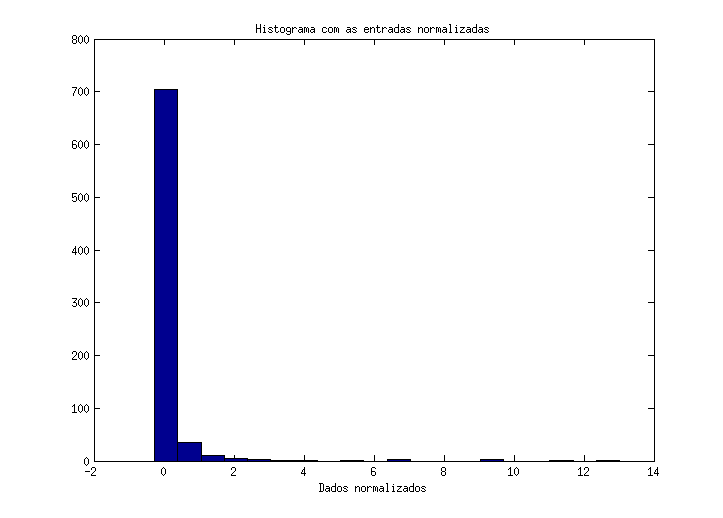
\includegraphics[width=0.65\textwidth]{image/hist_normalizados}
			  \caption{Dados normalizados.} 
			  \label{hist3}
	\end{figure}
	
	\FloatBarrier

\subsection{Variáveis participantes do modelo - Filtro de correlação}
 \label{sec:corr}

A fim de obter um resultado mais representativo nos preditores a serem
realizados, aplica-se um filtro de correlações nas 20 variáveis que inicialmente
foram propostas para determinar a precvisão do número de casos de dengue para a
próxima semana. Para isso, usamos o programa \texttt{calc\_corr2.m},
disponibilizado pelo professor. Obtem-se o gráfico mostrado na figura
\ref{fig:corr_variavel} a seguir:

	\begin{figure}[H]
			\centering
			  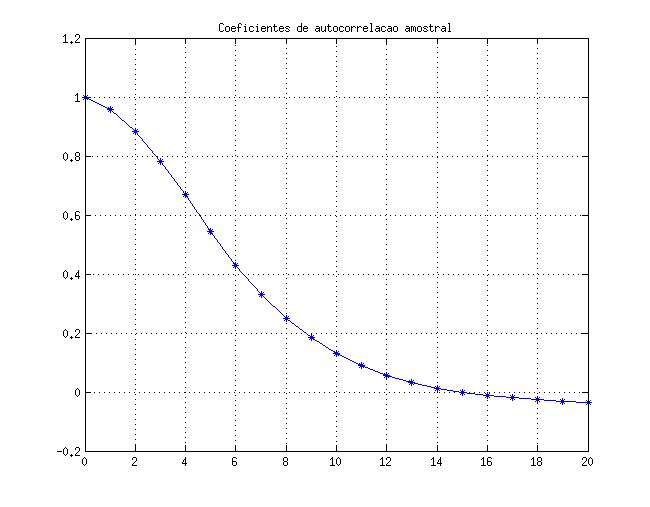
\includegraphics[width=0.60\textwidth]{image/corr_variaveis_preditor}
			  \caption{Correlação das 20 variavés escolhidas como entrada.} 
			  \label{fig:corr_variavel}
	\end{figure}
	
	\FloatBarrier
	
Observa-se neste gráfico que as cinco primeiras variáveis utilizadas no modelo
são as mais correlatas à saída. Em termos numéricos, as variáveis a partir da
sexta apresentam correlações inferiores a 0.5. Conclui-se, portanto, que em
termos de pertinência, as cinco variáveis iniciais são as mais importantes para
compor o valor a ser predito.

\subsection{Síntese de um preditor linear}
 
Para esta etapa, define-se \(M = 5\) a dimensão do espaço de entrada (consultar
seção \ref{sec:corr}) e \(R = 1\), a de saída. Em outras palavras, utilizaremos
dados de 5 semanas anteriores para determinar o resultado da 'semana seguinte'. As funções
utilizadas para a construção da série e nos cálculos dos preditores encontram-se, respectivamente, nos
programas \ref{lst:geracao} e \ref{lst:preditor} na seção
\textbf{Anexos} no fim deste documento.

\vspace{12pt}

Utilizaremos a estratégia de \textit{k-folds cross-validation} para estimar o
melhor valor do parâmetro \(c\). Neste caso, adota-se \(k=10\).

\subsubsection{Caso não regularizado}

A resolução de \(\overrightarrow{b} = \left( A^T A \right) A^T
Y\) utilizando apenas o conjunto de treinamento produz o vetor, cujos
coeficientes encontram-se na tabela abaixo, e um erro quadrático médio de
\textbf{0.2500}.

\[
\overrightarrow{b}_{nreg}^T = \begin{bmatrix}
  -0.1714 & 0.2349 & -0.3289 & -0.0528 & 1.2298 & -0.0000
  \end{bmatrix}
\]

\FloatBarrier
\subsubsection{Caso regularizado}

A utilização de um parâmetro \(c\) adicional e da estratégia \textit{k-fold
cross-validation} permite a adequação mais correta dos dados de entrada aos de
saída, conforme observado em sala de aula. A execução do programa
\texttt{resolve\_sistema\_k\_folds.m} da seção \textbf{Anexos} gera o gráfico,
em escala semi logarítmica, contido na figura \ref{fig:pred.regula}, que
relaciona \(c\) com a média do erro quadrático médio em cada uma das 10
execuções do programa (uma execução para cada uma das pastas de validação).

	\begin{figure}[H]
	  \centering
	  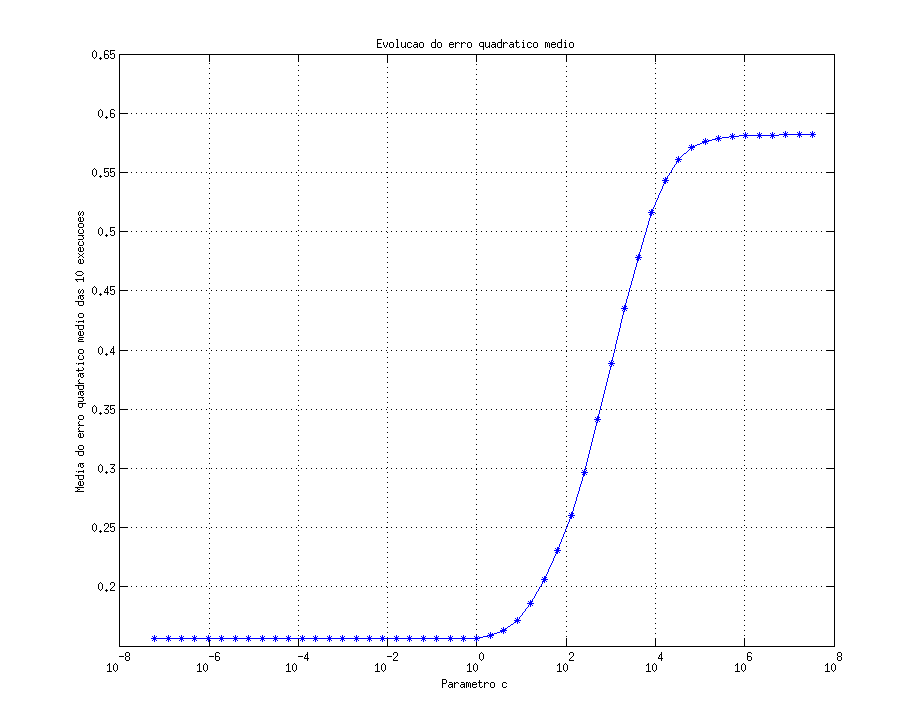
\includegraphics[width=0.65\textwidth]{image/preditor_regularizado_k_folds}
	  \caption{Erro quadrático médio em função do parâmetro c.} 
	  \label{fig:pred.regula}
	\end{figure}
	
	\FloatBarrier 
	
	Ressalta-se a presença de um mínimo local, para \(c_1 = 2^{-1} =
	0.5\), valendo \textbf{0.15602}. Esse erro é inferior a aquele obtido
	ao caso não regularizado, já que o preditor obtido
	neste caso adapta-se melhor a todo conjunto dos dados e não somente a aqueles
	que só foram usados no treinamento.
	
	\vspace{12pt}
	
	Enfim, explicitamos os vetores \(\overrightarrow{b}\) para \(c = 2^{-1}\):
	\FloatBarrier
	\begin {table}[H]
\centering
	\begin{tabular} {| c | c | c | c | c | c | c |}
	\hline 
	\( \overrightarrow{b}_1 \) & -0.1673 & 0.2193 & -0.3182 & -0.0397 & 1.2160 & 
	0.0023 \\\hline 
	\( \overrightarrow{b}_2 \) &-0.1685 & 0.2244 & -0.3230 & -0.0418 & 1.2195 &  0.0014
	\\ \hline 
	\( \overrightarrow{b}_3 \) & -0.1669 & 0.2195 & -0.3199 & -0.0379 & 1.2158 & 
	0.0015 \\ \hline 
	\( \overrightarrow{b}_4 \)  &-0.1674 & 0.2194 & -0.3185 & -0.0390 & 1.2155 & 
	0.0025 \\ \hline
	\( \overrightarrow{b}_5 \) & -0.1680 & 0.2217 & -0.3191 & -0.0400 & 1.2164 & 
	0.0008 \\ \hline 
	\( \overrightarrow{b}_6 \) & -0.1675 & 0.2199 & -0.3191 & -0.0390 & 1.2159 & 
	0.0018 \\ \hline 
	\( \overrightarrow{b}_7 \) & -0.1662 & 0.2329 & -0.3552 & -0.0222 & 1.2199 &
	-0.0014 \\ \hline 
	\( \overrightarrow{b}_8 \) & -0.1676 & 0.2352 & -0.3412 & -0.0347 & 1.2221 & 
	0.0008 \\ \hline 
	\( \overrightarrow{b}_9 \) &-0.1664 & 0.2202 & -0.3225 & -0.0365 & 1.2160 & 
	0.0009 \\ \hline 
	\( \overrightarrow{b}_{10} \) & -0.0832 & -0.0739 & 0.1328 & -0.1357 & 1.0721 &
	-0.0105 \\ \hline
	

	\end{tabular} 
\end {table}

Destaca-se que os valores para as componentes de uma mesma coluna não apresentam
uma grande variação entre si, isto é, os coeficientes do modelo autoregressivo
que produzem o menor erro médio possuem um comportamento bem definido.

\subsection{Síntese de uma rede neural MLP}
\label{sec:mlp}

Os resultados contidos nas seções \ref{sec:iteracoes} e \ref{sec:neuronios}
foram obitdos do programa \texttt{numberNeuronsMLP.m}, contido no trecho de
código \ref{lst:mlp} na seção \textbf{Anexos} no fim deste documento. Em poucas
palavras, este programa automatiza o processo de treinamento de análise dos
resultados de uma rede MLP para diferentes quantidades de neurônios e iterações.
Ele utiliza as funções disponibilizadas pelo professor, que foram adaptadas
somente para receber parâmetros de entrada no lugar de requirir os dados ao
usuário. Neste programa, há dois laços: o mais externo é reponsável por
modificar o número de iterações do algoritmo otimizador, escolhendo valores no
conjunto \(i \in \left\{ 50, 100, 150, 200, 300, 400 \dots 1000 \right\} \) e o
mais interno, o número de neurônios na camada intermediária no conjunto \( n \in
\left\{ 5, 6, 7 \dots 20 \right\} \). Para cada valor de \(i\) e de \(n\)
treina-se 10 MLPs (uma para cada configuração das \textit{folds}) e calcula-se
as médias dos seus desempenhos. Após obtermos as MLPs para todos os valores de \(n\), construimos
um gráfico com as médias dos erros de validação e de teste e, após todos os
valores de \(i\), desenhamos um último gráfico, com os desempenhos médios para
cada valor de \(i\). As próximas seções serão dedicadas às devidas explicações
sobre os resultados.

\subsubsection{Determinação do número de iterações}
\label{sec:iteracoes}

A figura \ref{fig:avg_iter} mostra um gráfico que relaciona o desempenho médio
das MLPs com o número de iterações. Observa-se que os comportamentos dos erros
de teste e de validação são similiares, isto é, quando uma apresenta um valor
elevado, a outra também apresentará. Esta afirmação explica-se pela capacidade
de generalização das MLPs: se uma rede é treinada de forma que o conjunto de
validação seja utilizado, é possível atingir um maior grau de flexibilidade a
todos os dados e, assim, o erro para dados novos não levados em consideração
(como aqueles do conjunto de teste) não se distanciará fortemente do erro de
validação. Sendo assim, utilizaremos o valor que possui o maior custo benefício
entre os dois erros, isto é, \(i = 1000\), que produz um erro médio de validação
igual a \textbf{0.1588} e um erro médio de teste valendo \textbf{0.1813}.

\begin{figure}[H]
			\centering
			  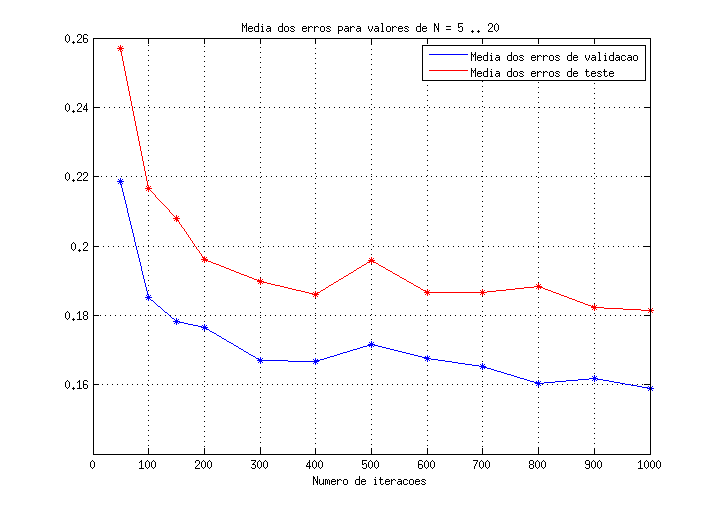
\includegraphics[width=0.650\textwidth]{image/mlp_average_iterations}
			  \caption{Média de todas as MLPs, calculadas para todo valor de \(n\), para
			  cada \(i\).}
			  \label{fig:avg_iter}
	\end{figure}
	
	\FloatBarrier

\subsubsection{Determinação do número de neurônios na camada intermediária}
\label{sec:neuronios}

Uma vez determinado o melhor número de iterações, é possível estabelecer o
número de neurônios que melhor se adequa à aplicação. Para isso, utilizamos o
gráfico da figura \ref{fig:iter1000}.


	\begin{figure}[H]
			\centering
			  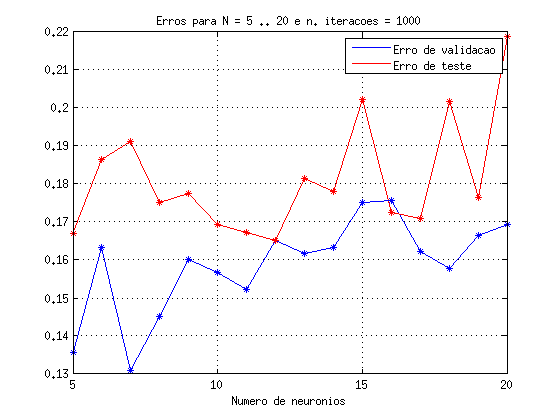
\includegraphics[width=0.650\textwidth]{image/mlp_1000_iterations}
			  \caption{Média de todas as MLPs, calculadas para cada valor de \(n\),
			  para \(i=1000\).}
			  \label{fig:iter1000}
	\end{figure}
	
	\FloatBarrier
	
O melhor custo benefício entre os dois erros é, neste caso \(n = 5\),
apresentando erro médio de validação de \textbf{0.1356} e erro médio de teste de \textbf{0.1671}.
Destaca-se que, para \(n=7\), temos o valor mínimo do erro de validação, mas, ao
mesmo tempo, um erro relacionado ao teste muito elevado. Por esta rezão, este
número de neurônios não foi escolhido.  Observa-se também que as duas curvas não
apresentam comportamentos definidos, isto é, os erros para diferentes valores de
\(n\) são muito distintos entre si.

\vspace{12pt}

Os demais resultados para outros valores de \(i\) e \(n\) podem ser observados
na figura \ref{fig:iens} na seção \textbf{Anexos}. 


\subsection{Síntese da Máquina de Aprendizado Máximo - \textit{ELM}}
\label{sec:elm}

Neste exercício, adotaremos uma \textit{ELM} com apenas uma camada
intermediária com um número de neurônios que determinaremos a seguir. Para tal,
utilizamos o programa \ref{lst:elm}, presente no fim deste documento na seção
\textbf{Anexos}. Neste trecho de código, iteramos o número de neurônios no
conjunto  \( \left\{ 100, 150, 250, 400, 500, 1000  \right\} \) e o parâmetro
regularizador \(c\) e, obtemos um gráfico da média do erro quadrático médio de
validação das 10 execuções (uma para cada \textit{fold}) para valor do número
de neurônios utilizado.

\vspace{12pt}

Após a execução no ambiente MATLAB, encontrou-se que o menor erro quadrático
médio junto ao conjunto de validação foi \textbf{0.3036}, referente a \(N =
400\) neurônios e \(c=2^{-6}=0.015625\). A figura a seguir mostra o resultado da
execução nestas configurações:

	\begin{figure}[H]
			\centering
			  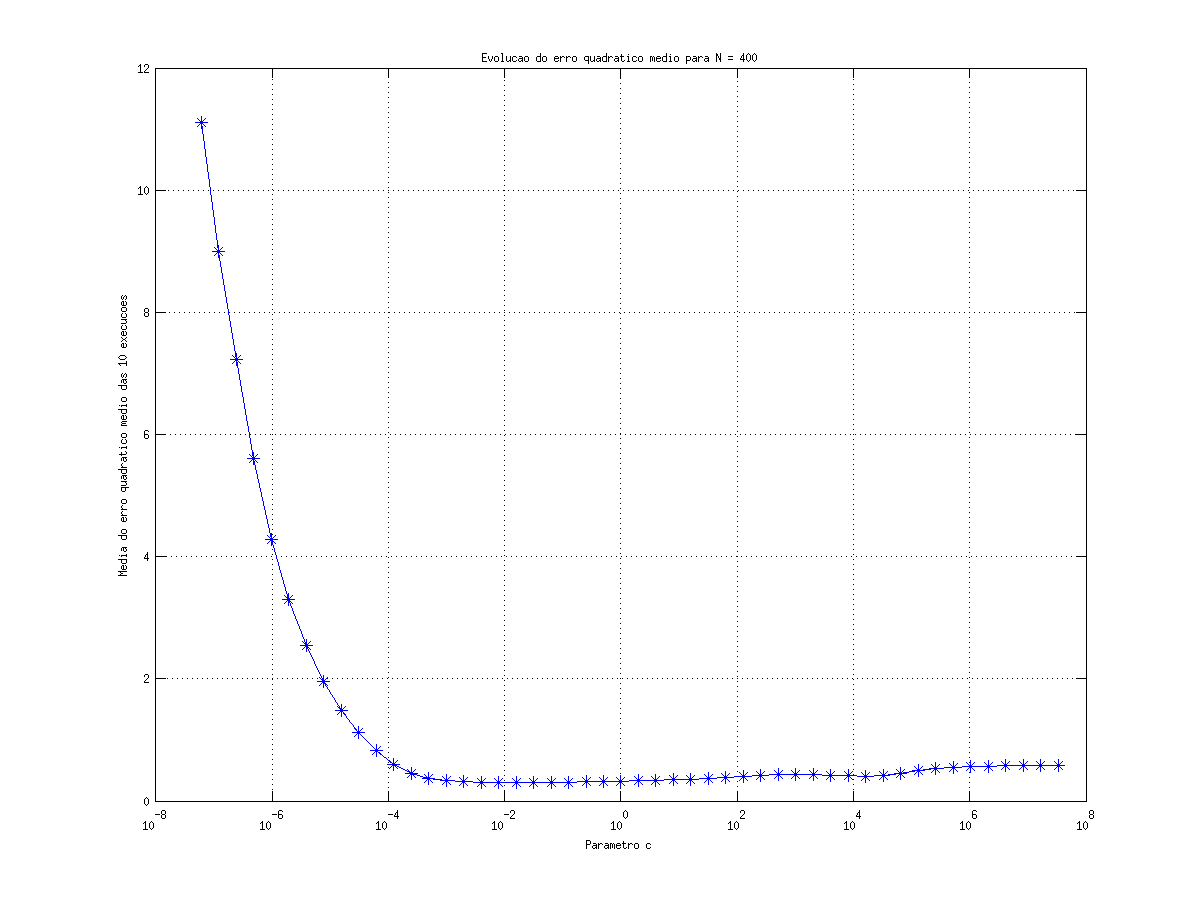
\includegraphics[width=0.650\textwidth]{image/elm_400_neurons}
			  \caption{Erro quadrático médio de validação em função de \(c\),
			  para \(N=400\).}
			  \label{fig:elm400}
	\end{figure}
	
	\FloatBarrier
	
Percebe-se que o erro cresce à medida que \(c\) se aproxima de 0 e depois se
estabiliza para c tendendo a infinito.  Os resultados das demais execuções
encontram-se na figura \ref{fig:elms} na seção \textbf{Anexos}.

\subsection{Análise dos resultados dos preditores lineares, MLPs e ELMs}
\label{sec:comparacao}

A pior performance entre os quatro preditores implementados nesta lista foi a
do \textit{ELM}, que obteve um erro quadrático médio de \textbf{0.3036}. Tal
resultado é um tanto quanto surpreendente, já que esse desempenho é inferior a
aquele dos preditores lineares, fato este que não era esperado.  Possíveis
explicações para este fato são a quantidade insuficiente de camadas utilizadas,
a inicialização dos pesos sinápticos da camada intermediária, que, foi neste
caso, determinada aleatoriamente segundo uma lei normal de média 0 e variância
1, ou algum erro eventual no programa \ref{lst:elm}.

\vspace{12pt}

O terceiro lugar, \textit{preditor linear não regularizado}, para qual só foi
utilizado o conjunto de treinamento para o cálculo do erro quadrático médio,
obteve um erro de \textbf{0.2500}. Uma vez o conjunto de validação não foi
utilizado, a capacidade de generalização do preditor é comprometido e, assim, o
preditor apresenta um erro relativamente alto.

\vspace{12pt}

Em segundo lugar, destaca-se \textit{preditor linear regularizado}, cujo erro
quadrático médio vale \textbf{0.15602}. A introdução de um parâmetro \(c\) adicional e a
sua determinação ótima juntamente ao conjunto de validação provaram que o
desempenho obtido pode ser melhorado de maneira significativa, visto que o
modelo linear mantem-se o mesmo. Isso significa que nesta oportunidade,
observa-se uma maior flexibilidade do preditor a todos os dados.

\vspace{12pt}  

Enfim, para o caso das MLPs, obtem-se um erro médio quadrático de validação de
\textbf{0.1356}, para \(i=1000\) e \(n=5\). É necessário dizer que este resultado foi
conseguido com base em uma quantidade de processamento muito superior aos dois
casos precedentes, uma vez que, no total, foram treinadas
\(10*\mathbf{card}(n)*\mathbf{card}(i) = 10*15*12 = 1800\) MLPs (uma para cada
configuração das \textit{folds}, cada valor de \(n\) e \(i\)). Foram utilizados
conjuntos de validação e teste para otimizar ainda mais a adequação da rede aos
dados. A rede neural é, portanto, a melhor opção para predizer a série temporal
da dengue em São Paulo.